\section{Analisi della dipendenza tra le variabili}

\subsection{Analisi di correlazione}
\begin{figure}[H]
	\centering
	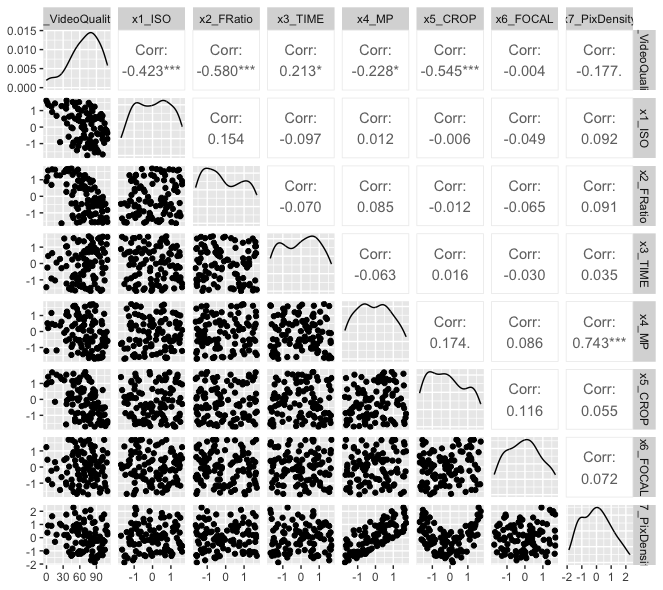
\includegraphics[width=0.90\textwidth]{../graphs/DescriptiveStatisticPlots/ggplot}
	\caption{Scatter plot delle variabili presenti nel dataset.}
	\label{fig:scatter}
\end{figure}

Dalla Figura~\ref{fig:scatter} si osserva, anche tramite i coefficienti di correlazione, una relazione lineare particolarmente evidente tra le variabili:
\begin{itemize}
	\item \textbf{x4\_MP} e \textbf{x7\_PixDensity}
\end{itemize}

Sono invece presenti relazioni di natura non lineare che non risultano ben descritte dal solo coefficiente di correlazione lineare. In particolare, tali dipendenze emergono tra:
\begin{itemize}
	\item \textbf{y\_VideoQuality} e \textbf{x1\_ISO}
	\item \textbf{y\_VideoQuality} e \textbf{x2\_FRatio}
	\item \textbf{y\_VideoQuality} e \textbf{x3\_TIME}
	\item \textbf{y\_VideoQuality} e \textbf{x5\_CROP}
	\item \textbf{x5\_CROP} e \textbf{x7\_PixDensity}
\end{itemize}

\subsection{Analisi di regressione}
Per analizzare la relazione tra la variabile \texttt{y\_VideoQuality} e ciascuna variabile indipendente, sono state effettuate regressioni semplici considerando prima i termini al primo grado.

\begin{table}[H]
	\centering
	\begin{tabular}{|c|c|}
		\hline
		\textbf{Variabile indipendente} & \textbf{p-value} \\
		\hline
		x1\_ISO & $1.17 \times 10^{-5}$ \\
		\hline
		x2\_FRatio & $2.63 \times 10^{-10}$ \\ 
		\hline
		x3\_TIME & $3.31 \times 10^{-2}$ \\
		\hline
		x4\_MP & $2.27 \times 10^{-2}$ \\
		\hline
		x5\_CROP & $4.39 \times 10^{-9}$ \\
		\hline
		x6\_FOCAL & $0.97$ \\
		\hline
		x7\_PixDensity & $0.0775$ \\
		\hline
	\end{tabular}
	\caption{P-value delle regressioni semplici con i termini al primo grado.}
	\label{tab:reg_lin_1grado}
\end{table}

Dalla Tabella~\ref{tab:reg_lin_1grado} si nota che i regressori \texttt{x1\_ISO}, \texttt{x2\_FRatio}, \texttt{x3\_TIME} e \texttt{x5\_CROP} risultano significativamente correlati con la variabile risposta, mentre gli altri non sembrano presentare una dipendenza lineare rilevante.

L’analisi è stata poi ripetuta considerando i termini quadratici delle variabili indipendenti:

\begin{table}[H]
	\centering
	\begin{tabular}{|c|c|}
		\hline
		\textbf{Variabile indipendente} & \textbf{p-value} \\
		\hline
		x1\_ISO & $2.46 \times 10^{-3}$ \\
		\hline
		x2\_FRatio & $1.28 \times 10^{-3}$ \\ 
		\hline
		x3\_TIME & $0.3094$ \\
		\hline
		x4\_MP & $0.2899$ \\
		\hline
		x5\_CROP & $0.3680$ \\
		\hline
		x6\_FOCAL & $0.7700$ \\
		\hline
		x7\_PixDensity & $0.8038$ \\
		\hline
	\end{tabular}
	\caption{P-value delle regressioni semplici con i termini al secondo grado.}
	\label{tab:reg_lin_2grado}
\end{table}

Dalla Tabella~\ref{tab:reg_lin_2grado} emerge una significativa dipendenza quadratica della variabile \texttt{y\_VideoQuality} rispetto ai regressori \texttt{x1\_ISO} e \texttt{x2\_FRatio}, mentre gli altri non risultano significativi nemmeno al secondo grado.
